\chapter{From Climate Information to Knowledge: Evaluating LLM-Based Systems}

\noindent\textit{Parts of this chapter are based on the work \emph{``Augmenting Large Language Models with Climate Indicators Computation for the Next-Generation Climate Services''}, by \textbf{Grassi, J.}, Pantiukhin, D., Kuznetsov, I., Koldunov, N., Dragan, M., and von Hardenberg, J. The manuscript is currently under review at Climate Services, a journal of Elsevier.}

\vspace{0.5em}
\begin{center}
    \rule{0.5\textwidth}{0.4pt}
\end{center}
\vspace{0.5em}


The previous chapter examined the climate information encoded in the parameters of Large Language Models. The results showed that LLMs can reproduce broad climatological regularities and recall widely communicated climate facts, but cannot be considered reliable sources of local quantitative information. Their errors increase when questions require geographical specificity, and their ability to reproduce the global magnitude of climate change does not extend to its regional distribution. These limitations point towards a different role for language models in Climate Services: rather than acting as autonomous sources of scientific information, they can provide a natural language interface to authoritative documents, climate datasets, and analytical tools.

Systems that extend language models with these external resources are commonly referred to as \emph{Augmented Language Models} (ALMs). Augmentation may allow a model to retrieve scientific evidence, access geographical and sectoral information, query climate databases, or execute dedicated computational tools. This potentially improves its specificity and traceability while preserving the ability of the LLM to interpret user questions and communicate results in accessible language.

Access to external information does not, however, automatically produce a reliable Climate Service. Retrieved documents may be incomplete or only indirectly related to the question, data may refer to inappropriate spatial or temporal scales, and analytical tools may be configured using unsuitable parameters. Even when the underlying evidence is scientifically valid, the LLM may overinterpret the results, omit relevant limitations, or formulate recommendations that are not supported by the analysis. Augmentation therefore extends the capabilities of LLMs, but also creates a longer epistemic chain that must itself be evaluated.

This challenge is particularly important because many Climate Services require more than the retrieval of existing information. User questions often need to be translated into tailored climate indicators whose definitions and parameters depend on the location, sector, asset, threshold, and planning horizon under consideration. Producing such information normally requires several operations: interpreting the question, identifying an appropriate indicator, acquiring suitable climate data, configuring and executing the calculation, and contextualizing the results. Standard LLMs can support the linguistic aspects of this process, but they cannot perform the underlying scientific computations reliably through text generation alone.

The first contribution of this chapter is therefore XCLIM-AI, a proof-of-concept system that connects an LLM to \emph{xclim}, an established open-source framework for climate indicator computation. XCLIM-AI translates natural-language questions into computable analyses by retrieving relevant indicator definitions, selecting their parameters, executing them on climate model data, and incorporating the resulting evidence into a structured response. The numerical computation remains deterministic and reproducible, while the LLM provides the interface through which user needs are interpreted and the results are communicated.

The second contribution concerns the evaluation of these augmented systems. If different forms of augmentation provide access to different types of evidence, how do they affect the epistemic quality of the resulting Climate Service? To address this question, the chapter compares four systems representing progressively different augmentation strategies: a Plain LLM relying on parametric knowledge; XCLIM-AI, providing computational augmentation; ClimSight, providing geographical, sectoral, and climate context; and ClimSight-XCLIM, combining contextual augmentation with climate indicator computation.

Their responses are evaluated according to four dimensions derived from the requirements of Climate Services: \emph{relevance}, \emph{credibility}, \emph{uncertainty communication}, and \emph{actionability}. The evaluation combines assessments by human experts with an ensemble of LLM judges, making it possible to investigate both the effects of augmentation and the extent to which automated evaluation can reproduce human judgments.

Within the DIKW framework adopted throughout this dissertation, this chapter addresses the transition from climate information to decision-relevant knowledge. External sources and computational tools provide evidence, while the language model selects, interprets, and communicates that evidence in relation to a user question. The central issue is therefore no longer simply whether an LLM can generate a plausible answer, but whether the complete system produces knowledge that is appropriately grounded, transparent about its limitations, and usable within a specific decision context.


\section{Augmented Language Models for Climate Services}

\subsection{From Parametric to External Knowledge}

As shown above, systems designed to interact with external knowledge are commonly referred to as \emph{Augmented Language Models} (ALMs) \citep{mialon_augmented_2023}. 

One of the most widely adopted forms of augmentation is Retrieval-Augmented Generation (RAG) \citep{lewis_retrieval-augmented_2020,gao_retrieval-augmented_2024}. In a conventional RAG workflow, the documents forming the external knowledge base are divided into smaller passages and represented as numerical embeddings. When a user submits a question, the query is mapped into the same representation space and compared with the indexed passages. The most relevant passages are then retrieved and included in the prompt provided to the LLM, which uses them as evidence when generating the answer. More advanced implementations may also reformulate the query, combine semantic and keyword-based search, rerank the retrieved passages, or perform several retrieval iterations before producing the final response.

This architecture changes the provenance of the generated information. The response no longer depends exclusively on what the LLM has retained during training, but can be connected to identifiable sources. It also allows the knowledge base to be updated without retraining the model. For Climate Services, this is particularly valuable because scientific assessments, model projections, adaptation guidelines, and sector specific evidence evolve continuously and cannot be assumed to be fully represented in the training data of a general purpose LLM.

One of the first applications of this approach was ChatClimate, which connected GPT-4 to the reports of the IPCC Sixth Assessment Cycle \citep{vaghefi_chatclimate_2023}. The reports were divided into passages and indexed in a vector database; for each question, the system retrieved the passages with the greatest semantic similarity and supplied them to the model together with their corresponding references. The authors evaluated both a configuration constrained to the retrieved evidence and a hybrid configuration that combined IPCC information with the parametric knowledge of GPT-4. The latter produced more complete responses, while the retrieval component improved access to specific quantitative statements and allowed the system to associate its claims with identifiable sections of the IPCC reports. ChatClimate therefore demonstrated the potential of RAG to make authoritative assessments more accessible, but it remained primarily an interface to a predefined textual corpus.

ClimateGPT followed a complementary direction by combining external retrieval with adaptation of the language model itself \citep{thulke_climategpt_2024}. Rather than using an unmodified general-purpose model, ClimateGPT introduced a family of models trained on a large collection of climate related scientific material and subsequently tuned using examples developed with climate scientists. The models were further connected to a hierarchical retrieval system intended to provide more detailed evidence and reduce unsupported generation. This approach combines two distinct strategies: domain adaptation strengthens the parametric representation of climate concepts, while retrieval provides access to specific documents at inference time. Subsequent work on ClimateGPT nevertheless showed that retrieval alone does not ensure that the generated answer remains faithful to the retrieved material. The composition of the tuning data and the ability of the model to follow the supplied evidence also play an important role \citep{thulke_listen_2025}.

Other systems have narrowed the knowledge base to particular sectors and user communities. My Climate Advisor, for example, was developed to support climate adaptation in agriculture by retrieving evidence from peer-reviewed research and selected relevant grey literature \citep{nguyen_my_2024}. The system used open-source language models and generated answers accompanied by references, with particular attention to provenance, privacy, and the needs of agricultural practitioners. Its subsequent development into My Climate CoPilot expanded the platform and incorporated iterative evaluation by domain experts, including agricultural and climate specialists \citep{nguyen_my_2025}. These systems illustrate how the selection and curation of the external corpus can be tailored to a specific application rather than attempting to cover the climate domain in its entirety.

A related approach was adopted for the United Kingdom Climate Projections (UKCP). The UKCP chatbot was designed to answer questions using the UKCP18 archive as its authoritative source \citep{biswas_evaluating_2025}. Its development compared alternative strategies for document segmentation, query expansion, retrieval, and reranking, while explicitly constraining the generated answers to information available in the archive. This narrower design reduces the range of questions that the system can answer, but makes it possible to evaluate whether the response is faithful to an institutional Climate Service product. It also highlights that the quality of a RAG system depends not only on the language model, but on the complete retrieval pipeline through which relevant evidence is identified and presented to it.

While these systems primarily focus on scientific and technical documents, Climate Services generally require the combination of several heterogeneous sources. ClimSight was introduced to address this requirement by connecting a LLM interface to geographical information, model data, and scientific literature \citep{koldunov_local_2024,kuznetsov_transforming_2025}. Starting from a user question and geographical coordinates, specialized agents retrieve information on the location, environmental characteristics, historical hazards, relevant scientific literature, and projected climate conditions. A final component then synthesizes these contributions into a localized climate assessment. ClimSight therefore extends the RAG paradigm from the retrieval of passages within a single document collection to the coordination of multiple information sources, each contributing a different component of the final response.

More recent work has moved further towards the joint use of textual and numerical climate information. The regional Climate Service framework proposed by \citet{matsuoka_llm_2026}, for example, combines an LLM with RAG over scientific publications and local adaptation plans, as well as access to precomputed statistics derived from ensemble climate projections. User questions are translated into search conditions that identify the relevant location, climate variable, warming level, and statistical quantity, after which the corresponding numerical values are retrieved from structured tables. This allows the system to include quantitative regional projections in its answers while preserving efficient retrieval at inference time.

These developments show a gradual expansion in the scope of external knowledge available to LLM-based Climate Services. Early systems primarily grounded responses in authoritative reports; subsequent applications incorporated domain-specific literature, local documents, geographical databases, and numerical climate projections. The role of the LLM consequently evolved from summarizing retrieved passages to coordinating heterogeneous sources and contextualizing their content for a particular user and location.

Beyond extending the range of information available to the model, a further step is therefore required: validating whether and how these different forms of augmentation improve the epistemic quality of the resulting Climate Service. Access to additional documents, contextual data, or numerical projections does not necessarily make an answer more reliable or useful. The complete system must be evaluated to determine whether augmentation produces responses that are more relevant to the user, more credible in their evidential basis, more transparent about uncertainty, and more actionable within a specific decision context.

The following two subsections address these complementary developments. The first introduces computational augmentation as a means of moving beyond the retrieval of existing information towards the generation of tailored climate indicators through validated scientific tools. The second defines a framework for evaluating how computational, contextual, and combined augmentation strategies affect the epistemic quality of LLM-based Climate Services.


\section{Methods}

\subsection{System Architectures}

The evaluation compares four LLM-based systems: a Plain LLM, XCLIM-AI, ClimSight, and ClimSight-XCLIM. The Plain LLM requires no dedicated architectural description, as it consists of a standard prompted language model without access to external tools, retrieval systems, or climate data. ClimSight is included as an existing multi-agent climate-service system, and we refer to \citet{kuznetsov_transforming_2025} for its full architecture.

This section therefore focuses on the two configurations that introduce climate-indicator computation: XCLIM-AI as a standalone agent, and ClimSight-XCLIM, where the same agent is embedded within the ClimSight workflow.

\subsubsection{XCLIM-AI Architecture} \label{xclim-architecture}

XCLIM-AI is implemented as an autonomous LLM-based workflow that translates a user query into a set of computable climate indicators for a specific location and uses the resulting calculations to generate a structured response. The system combines two components (Figure~\ref{fig:xclim-architecture}): a retrieval module, which maps the query to relevant indicators from the xclim framework \citep{bourgault_xclim_2023}, and a tool-based module, which executes the corresponding indicator functions on climate model data and formats the results for response generation.

The Retrieval Augmented Generation (RAG) agent queries a vector-store containing both descriptions and technical specifications of climate indicators implemented in xclim. 
However, these indicator descriptions are concise and rely heavily on technical jargon, including variable names and Python parameter definitions, which complicates the task of matching user-friendly natural language queries with the most appropriate indicator. 
To address this issue, in this work we employed an advanced reasoning language model (OpenAI o3; \citet{openai_introducing_2025}) to rewrite the technical descriptions of xclim climate indicators into plain, application-oriented language (see Supplementary Material A for the prompt). 
The model emphasized what each indicator measures, why it matters, and how it supports risk assessment and decision-making, ensuring that the descriptions are directly relevant. The descriptions have then been embedded with OpenAI text-embedding-ada-002 \citep{openai_text-embedding-ada-002_2022}, that transformed each climate indicator description into a dense vector with 1536 dimensions.

When the agent is triggered by a human query (Figure \ref{fig:xclim-architecture-workflow}), the refiner first reformulates the query to emphasize elements that facilitate matching with relevant climate indicators. In parallel, it extracts a concise list of topics that must be addressed in the answer. The refined query is then embedded using text-embedding-ada-002, and the top-$k$ candidate indicators are retrieved from the vector store based on decreasing cosine similarity \citep{salton_developments_1991}. These indicators are passed to the evaluator node, which checks whether the initial query is adequately fulfilled and whether all extracted topics are covered. If the evaluation is negative, the system returns to the refiner with additional guidance to improve the reformulation, thus initiating a new iteration. The loop continues until either the evaluator concludes that the requirements are satisfied or the maximum number of iterations is reached. Finally, the aggregator reviews the set of retrieved indicators and selects those that best capture the intent of the query while ensuring coverage of the identified topics.

The selected indicators are then passed to the tool-calling component of the agent (Fig.~\ref{fig:xclim-architecture-workflow}), which executes the corresponding xclim functions. To compute the indicators, the agent retrieves daily climate data from an ensemble of seven CMIP6 High Resolution Model Intercomparison Project models (HighResMIP; \citet{haarsma_high_2016}) through the open-source Open-Meteo platform \citep{zippenfenig_open-meteo_2024}. The dataset covers the historical period 1950--2014 and the future period 2015--2050 under the high-emission SSP5-8.5 scenario \citep{oneill_scenario_2016}. Data are available over global land areas at a horizontal resolution of $0.1^\circ \times 0.1^\circ$, corresponding to approximately 10 km. The tool-calling component can access nine daily climate variables, listed in Table~\ref{tab:variables_openmeteo}. Climate data are retrieved point-wise: for each indicator computation, the requested indicator is calculated for the single grid cell corresponding to the selected location, representing an area of approximately $10 \times 10$ km.

\begin{table}[ht]
    \centering
    \caption{Variables obtained from Open-Meteo and derived variables}
        \begin{tabular}{llp{8.5cm}}
            \toprule
            \textbf{Variable} & \textbf{Source} & \textbf{Description / Method} \\
            \midrule
            \texttt{tasmax} & Open-Meteo & Daily maximum air temperature ($^\circ$C) \\
            \texttt{tas} & Open-Meteo & Daily mean air temperature ($^\circ$C) \\
            \texttt{tasmin} & Open-Meteo & Daily minimum air temperature ($^\circ$C) \\
            \texttt{pr} & Open-Meteo & Daily total precipitation (mm\,day$^{-1}$) \\
            \texttt{sfcWind} & Open-Meteo & Daily mean 10\,m wind speed (m\,s$^{-1}$) \\
            \texttt{sfcWindmax} & Open-Meteo & Daily maximum 10\,m wind speed (m\,s$^{-1}$) \\
            \texttt{hurs} & Open-Meteo & Daily mean relative humidity (fraction) \\
            \texttt{tdps} & Open-Meteo & Daily mean dew point temperature ($^\circ$C) \\
            \midrule
            \texttt{wb} & Derived & Water budget estimated as precipitation $-$ potential evapotranspiration (PET), where PET is derived with the Baier and Robertson method (BR65; \cite{baier_estimation_1965}) \\
            \bottomrule
        \end{tabular}
    \label{tab:variables_openmeteo}
\end{table}

When calling these functions, the tool caller is responsible for specifying all the parameters necessary for computing the indicators. For example, the \texttt{heat wave frequency} indicator counts events in which both daily minimum and maximum  temperatures exceed predefined thresholds over a specified number of consecutive days. Consequently, the agent must determine suitable values for parameters such as the thresholds of minimum and maximum temperatures, and minimum number of day based on its internal knowledge and any contextual clues present in the human query.

Once a tool is invoked, the system does not only return the raw output of the xclim indicator, but also computes a set of statistical summaries. 
These functions evaluate the indicator output across different periods (historical, short-term, medium-term), providing annual and, when applicable, monthly aggregations. 
The resulting metrics include mean, standard deviation, minimum, maximum, and Mann--Kendall trend  statistics \citep{gilbert_statistical_1987} (slope, intercept, and significance level). 
The structured dictionary of statistics is then passed to the LLM together with the indicator results, allowing it to reason over both the detailed time series and its condensed descriptors.

It is worth noting that the entire process of computing the indicators is deterministic and not delegated to the generative capabilities of the LLM, with the only exception being the selection of the parameters. During the computation of the climate indicators, the system also produces standardized images and log files containing the description of the parameters used, in order to ensure full reproducibility and transparency of the analysis.

Once all tools have been executed, the agent produces the final report. This report consists of indicator-specific sections with configuration details, numerical results, and comparisons across periods, followed by a synthesis that integrates the findings and discusses impacts and risks (Fig.~\ref{fig:xclim-architecture-example}).     

From a performance perspective, for each query, the system processes approximately 6k–10k tokens, of which roughly 300–800 correspond to model completion while the remainder is used for prompts circulating through the multi-step agentic pipeline. Using current cloud-model pricing, this corresponds to a per-query cost in the order of a few US cents for lightweight models (e.g., Gemini 3 Flash) and up to several tens of cents when high-end reasoning models (e.g., OpenAI GPT-5.2, Anthropic Claude Sonnet 4.5) are employed.

In addition to model inference, the system requires access to a Python environment with all necessary packages installed to compute the climate indicators. However, because XCLIM-AI operates on local time series extracted from HighResMIP rather than on large spatial datasets, the computational load is modest: typical indicator calculations involve arrays of daily data for one location and thus run efficiently on a standard CPU without requiring GPU acceleration or high-performance computing infrastructure. Memory requirements remain low (on the order of a few tens of megabytes), and execution time for each indicator is usually below a second. In the present configuration, the time series data are retrieved from the Open-Meteo weather API, and fetching a daily time series for a location typically takes on the order of a couple of seconds due to network latency and API response time.


\clearpage

\begin{figure}[p]
    \centering

    \begin{subfigure}{0.9\textwidth}
        \centering
        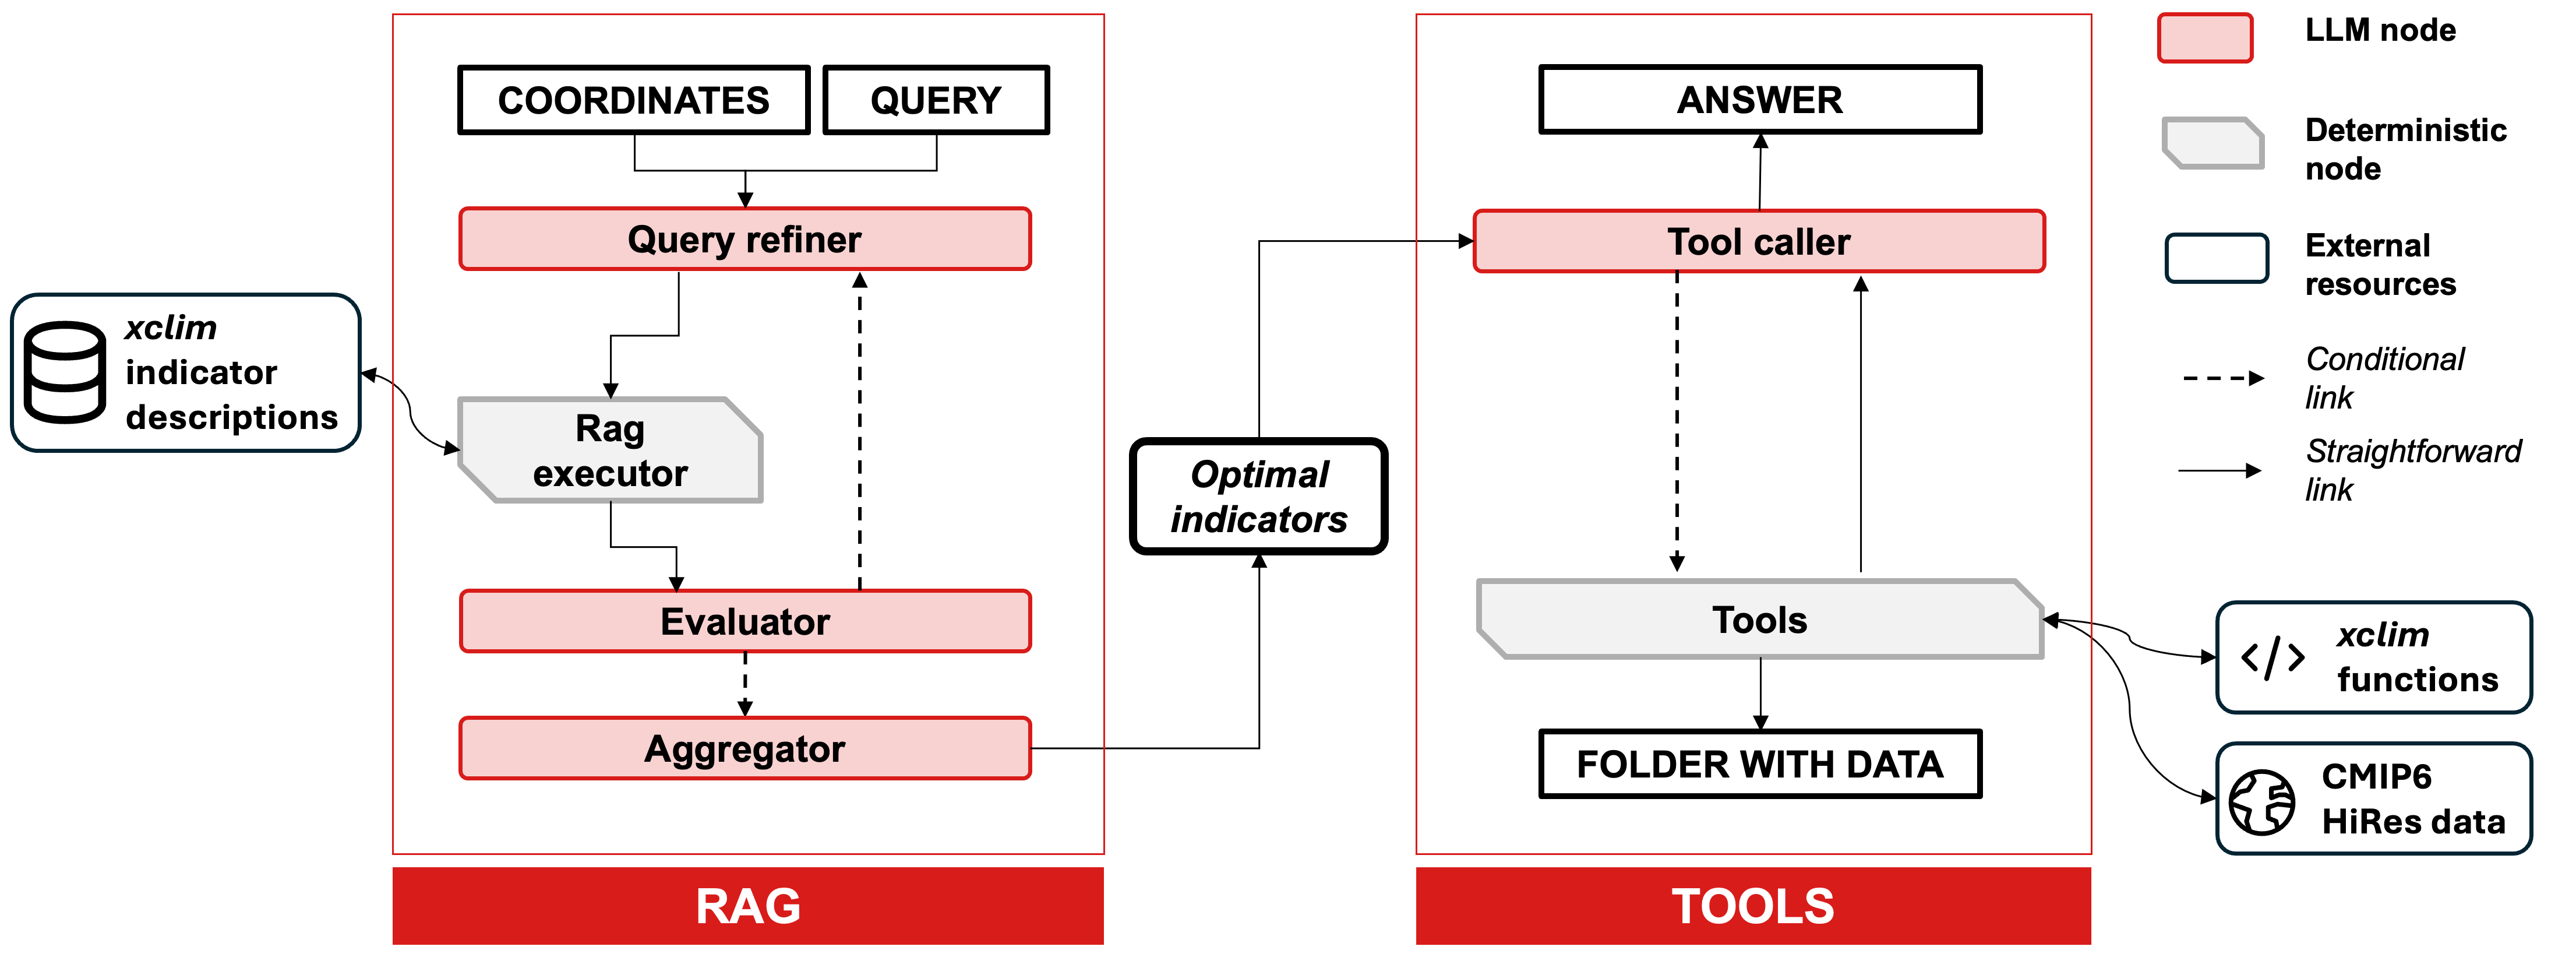
\includegraphics[
            width=\textwidth,
            height=0.34\textheight,
            keepaspectratio
        ]{Chapter5/figs/xclim-architecture.png}
        \caption{Architecture of XCLIM-AI.}
        \label{fig:xclim-architecture-workflow}
    \end{subfigure}

    \vspace{0.5cm}

    \begin{subfigure}{0.9\textwidth}
        \centering
        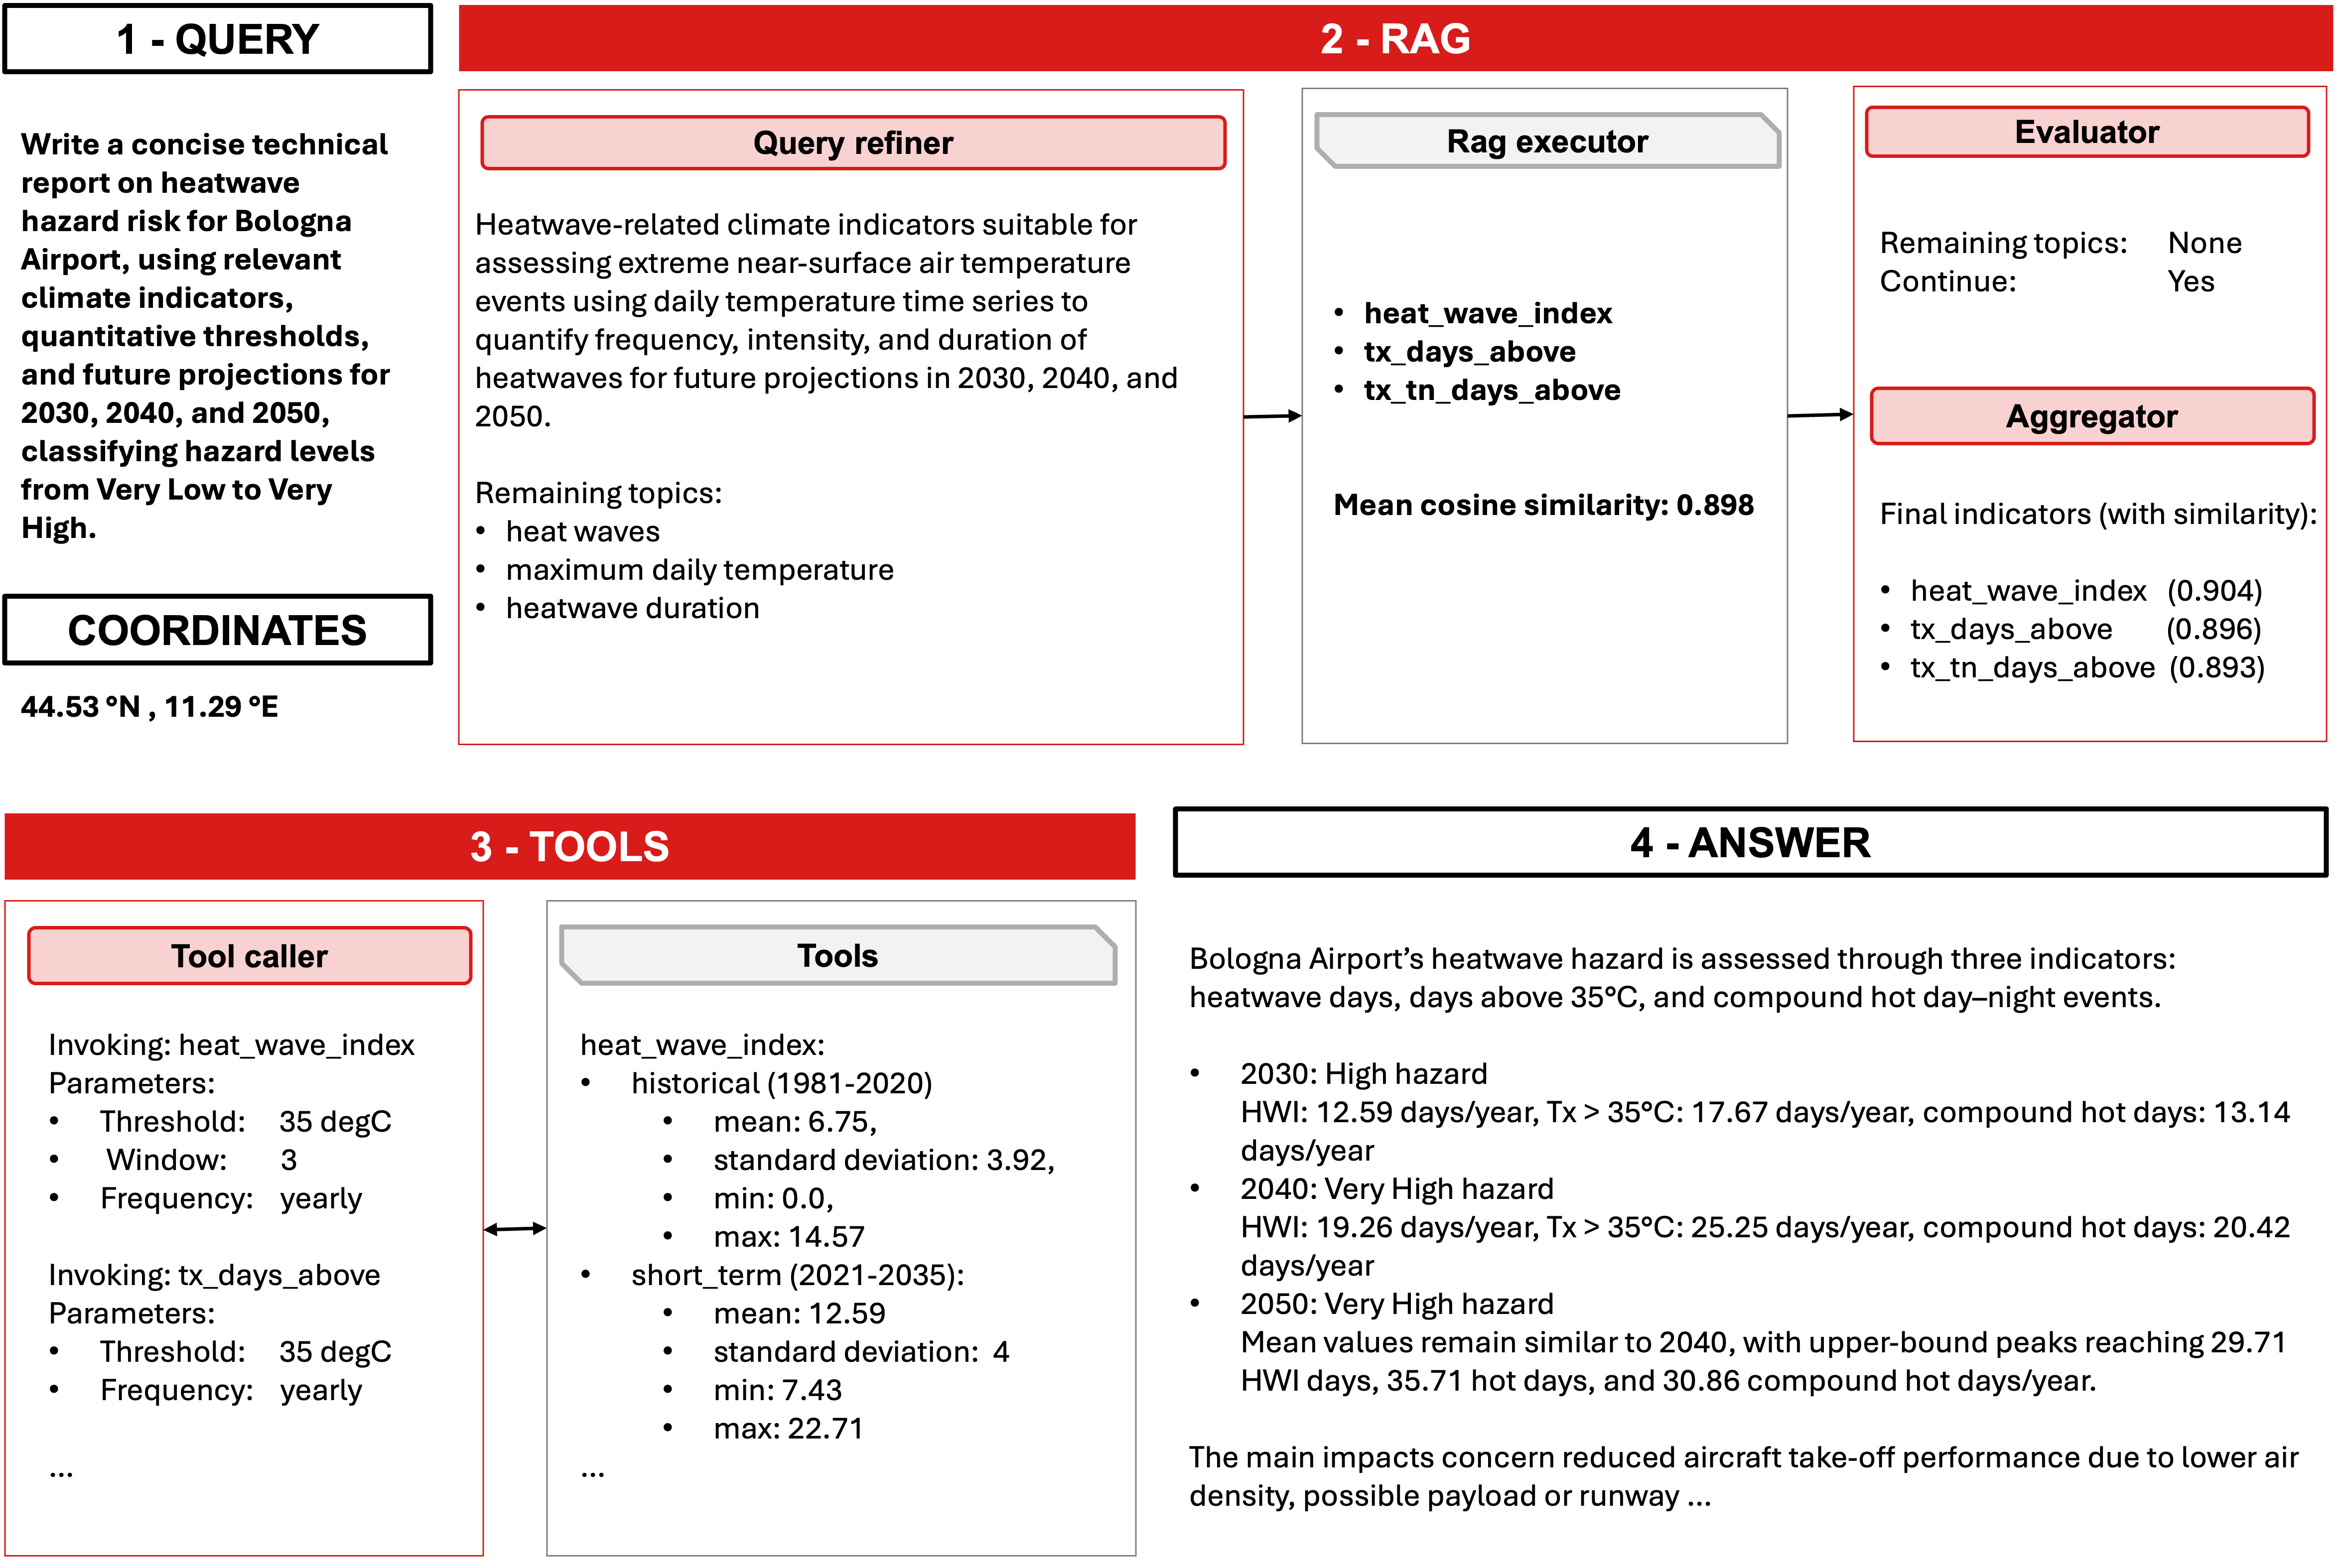
\includegraphics[
            width=\textwidth,
            height=0.34\textheight,
            keepaspectratio
        ]{Chapter5/figs/workflow.png}
        \caption{Example execution of the XCLIM-AI workflow.}
        \label{fig:xclim-architecture-example}
    \end{subfigure}

    \caption{
        Architecture and example execution of the XCLIM-AI workflow. Panel~(a) shows the overall architecture, combining a retrieval module that maps the user query to relevant \emph{xclim} indicators with a tool-calling module that executes the selected indicators on climate data and returns quantitative evidence for response generation. Panel~(b) illustrates an example execution in which the query is refined, matched to candidate indicators through retrieval-augmented generation, evaluated and aggregated, and finally passed to the tool-calling module for indicator computation
        and evidence-grounded answer generation.
    }
    \label{fig:xclim-architecture}
\end{figure}

\clearpage


\subsubsection{XCLIM-AI as a ClimSight Agent} \label{climsight-xclim}

\begin{figure}[H]
    \centering
    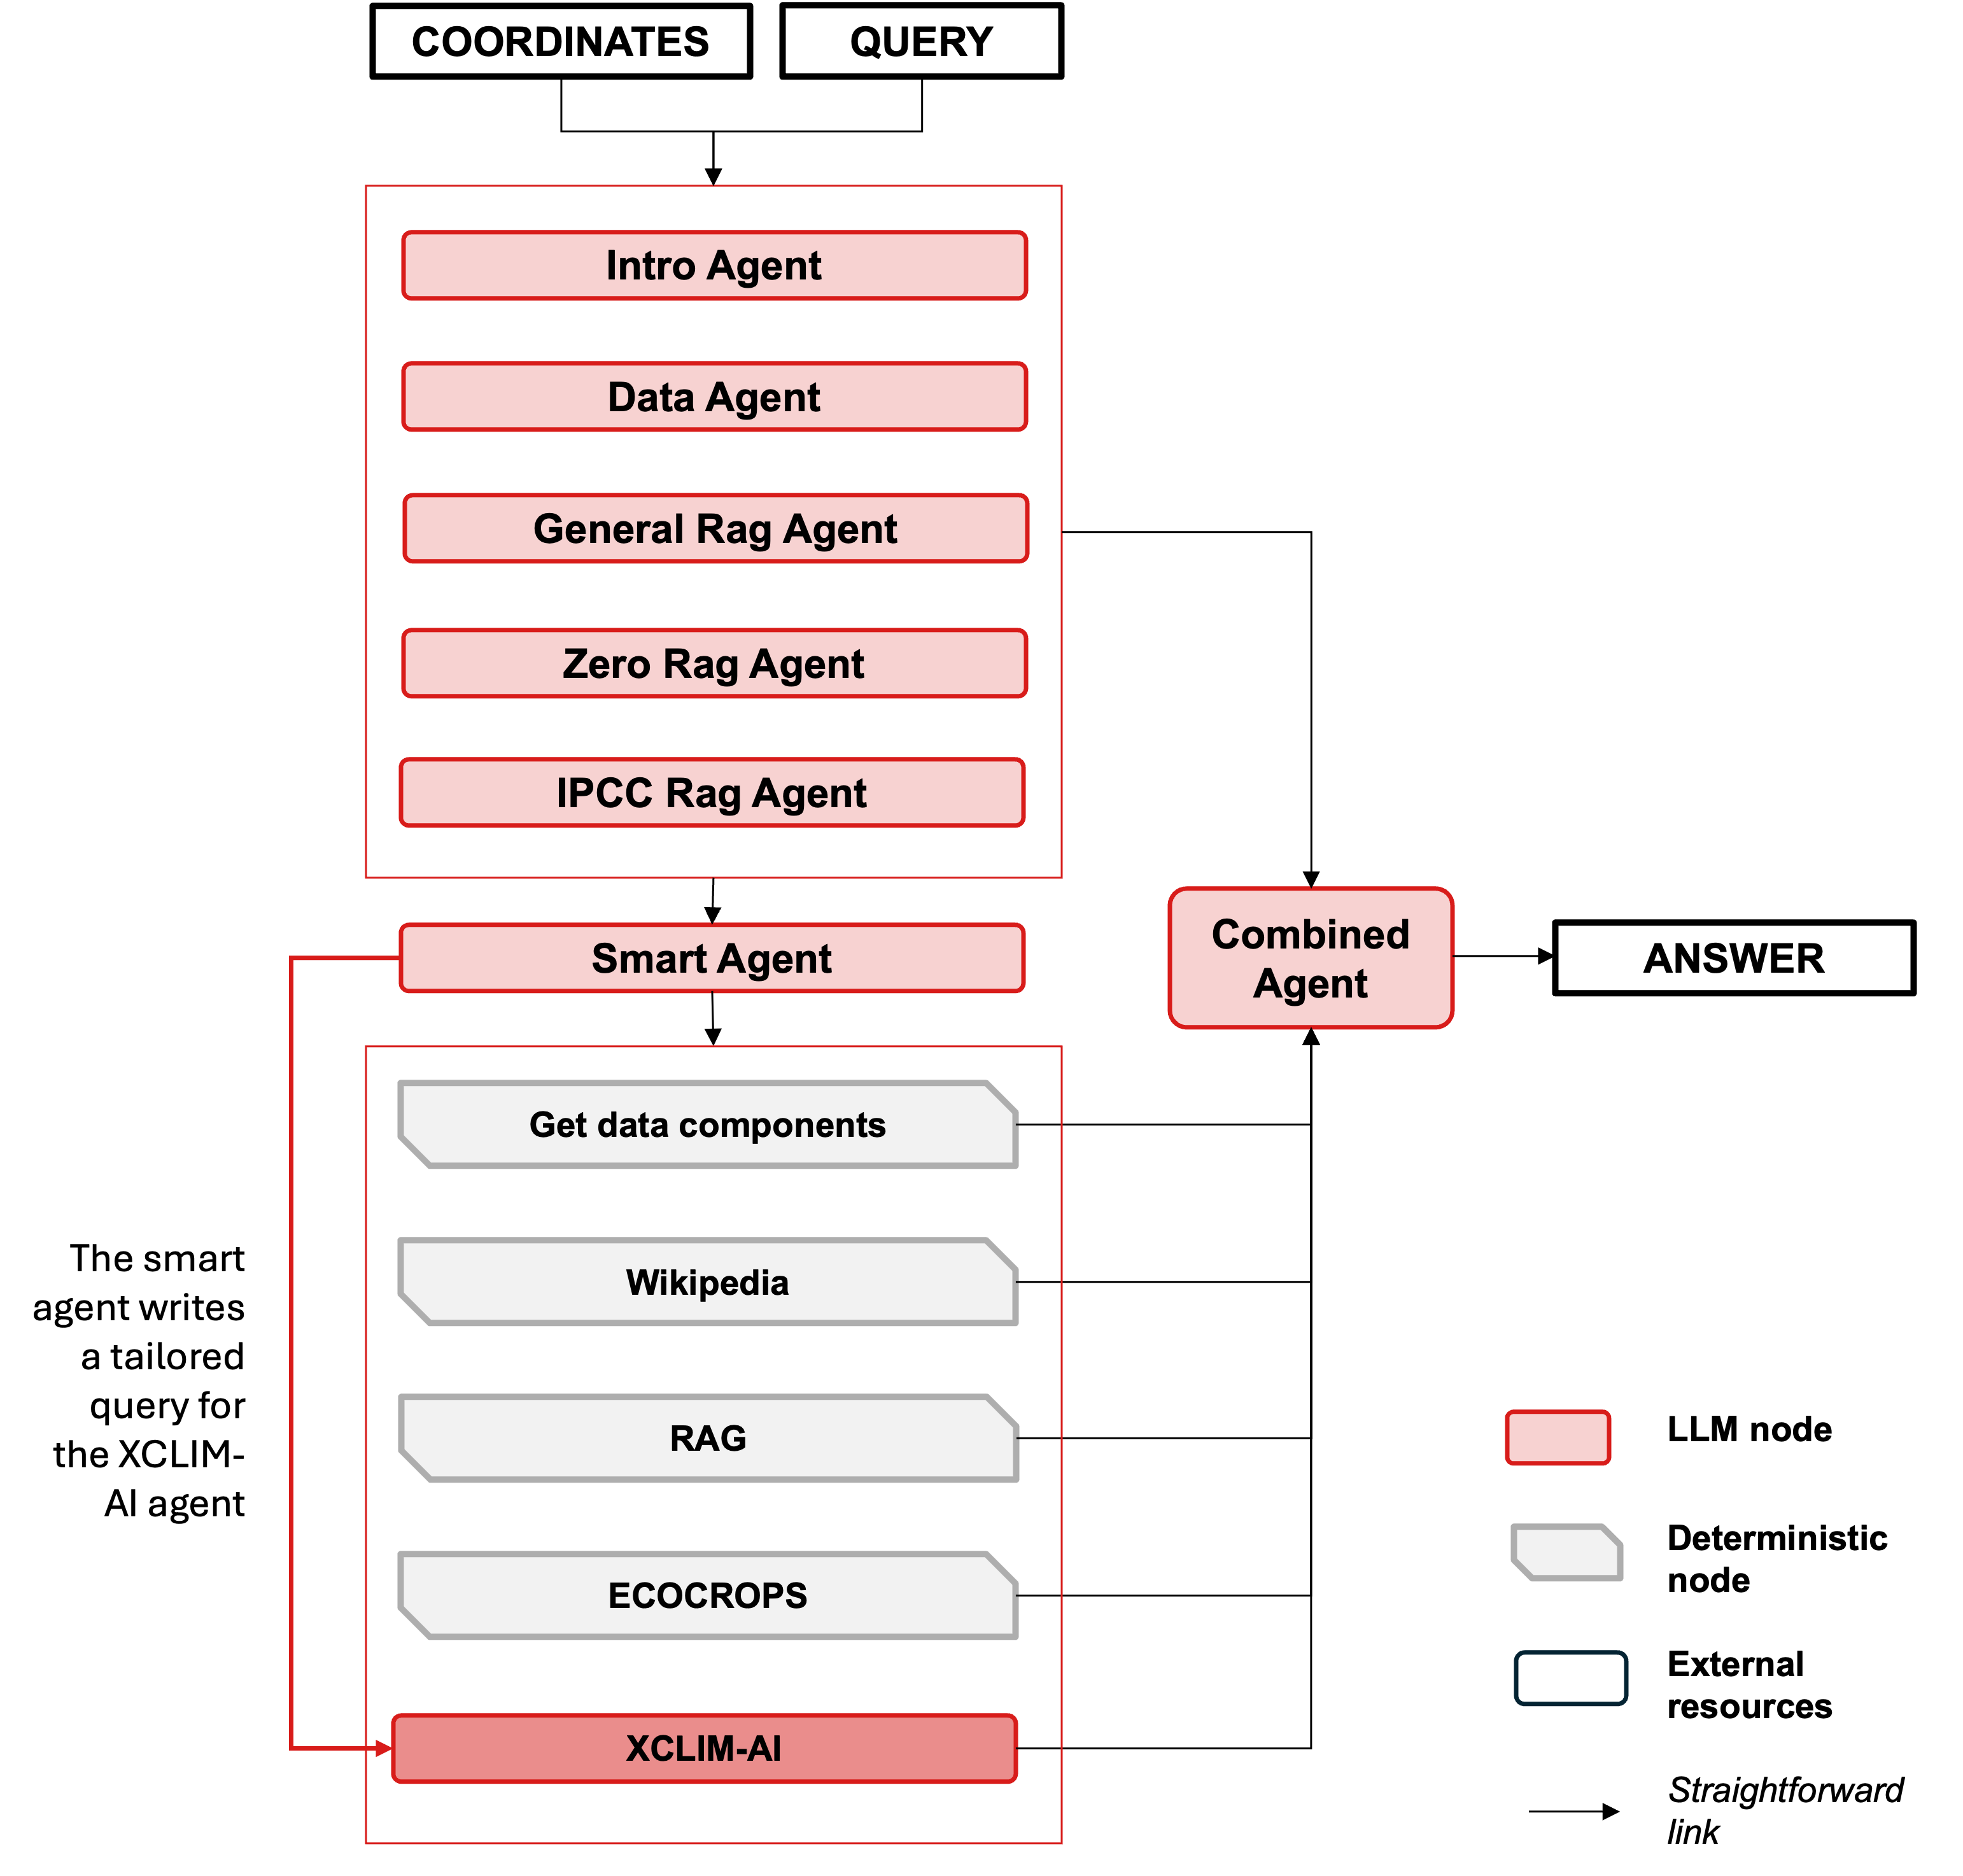
\includegraphics[width=0.75\linewidth]{Chapter5//figs/climsight-augmented.png}
    \caption{
    Architecture of ClimSight-XCLIM. XCLIM-AI is integrated as a callable component of the ClimSight smart agent, which formulates a tailored query for climate-indicator computation after the initial ClimSight agents have contextualized the user request.
    }
    \label{fig:climsight-xclim-architecture}
\end{figure}

ClimSight \citep{koldunov_local_2024, kuznetsov_transforming_2025} is an open-source agentic tool that integrates LLMs with geographical and climate data to provide localized climate information. Its modular design is based on LangGraph \citep{langchain_langgraph_2024} and LangChain \citep{langchain_langchain_2023}, and enables tailored analyses for different application domains while supporting interoperability with other systems.

By default, ClimSight employs five agents for analyzing the query, retrieving climatological data from a kilometer-scale model \citep{rackow_multi-year_2025}, and performing RAG over sectoral literature (Fig.~\ref{fig:climsight-xclim-architecture}). An additional agent, called the smart agent, can access external tools and refine queries for the RAG process.

We deployed XCLIM-AI, in the configuration described in the previous section, as a callable for the smart agent. This means that XCLIM-AI is invoked after ClimSight has already processed a substantial amount of information. Therefore, the smart agent can tailor a query for the XCLIM-AI agent that already incorporates insights from the previous analysis, ideally making the selection and computation of the appropriate climate indicator more efficient.

\subsection{Evaluation Design} \label{methods_evaluation_design}
\subsubsection{Evaluation dimensions} \label{evaluation-dimensions}

We evaluate system outputs along four dimensions: relevance, credibility, uncertainty communication, and actionability. These dimensions were selected because Climate Services requires information to be tailored to the user and decision context, scientifically trustworthy, explicit about limitations and uncertainty, and useful for adaptation planning and action \citep{lemos_narrowing_2012, hewitt_global_2012, vaughan_climate_2014, jahan_assessing_2023, boon_defining_2024, boon_developing_2025}. They also reflect the broader literature on usable knowledge, where the value of scientific information for decision-making is commonly associated with salience, credibility, and legitimacy \citep{cash_knowledge_2003, dilling_creating_2011, mcnie_delivering_2013}.

\paragraph{Relevance.}
Relevance refers to the extent to which the response addresses the user's question, location, sector, and decision context. In Climate Services, information is rarely useful in the abstract: the same climate variable or indicator may have different meanings depending on the asset, exposure, vulnerability, planning horizon, and adaptation problem considered. For this reason, Climate Service evaluation frameworks emphasize the need for information that is tailored to users' needs, problems, and decision-making contexts \citep{vaughan_climate_2014, jahan_assessing_2023, boon_developing_2025}. In the context of LLM-based systems, relevance therefore measures whether the answer moves beyond generic climate statements and selects evidence, indicators, spatial references, and impacts that are appropriate for the specific query.

\paragraph{Credibility.}
Credibility refers to the perceived scientific adequacy, trustworthiness, and evidential grounding of the response. Climate Services are expected to rely on scientifically sound information and expertise, but credibility also depends on whether users can understand why a conclusion should be trusted \citep{hewitt_global_2012, vaughan_climate_2014}. This is particularly important for LLM-based systems, whose responses may be fluent and authoritative while lacking traceable evidence or reproducible analytical support. We therefore assess credibility not only as factual plausibility, but as the degree to which the response is supported by identifiable sources, transparent reasoning, appropriate use of data, and scientifically valid procedures. This criterion is closely related to the literature on usable science, where credibility is one of the core attributes that enables knowledge to inform decisions \citep{cash_knowledge_2003, dilling_creating_2011, mcnie_delivering_2013}.

\paragraph{Uncertainty communication.}
Uncertainty communication refers to the extent to which the response explicitly acknowledges, qualifies, and communicates the limitations of the information provided. Climate information is inherently uncertain because it depends on observational constraints, model structure, internal variability, emission scenarios, downscaling choices, spatial resolution, and indicator definitions. For adaptation decisions, these uncertainties should not simply be omitted or treated as a weakness; rather, they should be communicated in ways that help users interpret the robustness, range, and conditional nature of the evidence \citep{boon_defining_2024, boon_developing_2025}. In our evaluation, this criterion captures whether the answer makes clear what assumptions are involved, and how these uncertainties affect the interpretation of the results.

\paragraph{Actionability.}
Actionability refers to the degree to which the response can support concrete adaptation reasoning, planning, or decision-making. A Climate Service output may be scientifically correct and relevant, yet still have limited practical value if it does not help users understand implications, compare options, identify risks, or frame possible responses. The Climate Services literature increasingly emphasizes that successful services should contribute to better decisions, increased user capacity, and tangible or intangible benefits for adaptation \citep{lemos_narrowing_2012, vaughan_climate_2014, boon_successful_2022, boon_developing_2025}. In the context of LLM-based responses, actionability therefore evaluates whether the answer translates climate evidence into decision-relevant implications, such as adaptation priorities, risk thresholds, affected activities, or planning considerations, while avoiding unsupported prescriptions.

\subsubsection{Evaluation set-up} \label{evaluation-set-up}
These dimensions are evaluated over the answers that different LLM systems give to 50 climate-related questions from \citep{kuznetsov_climsight-gpt41-mini-climate-assesments_2025}. The dataset focuses on localized questions related to climate change adaptation, each categorized into thematic domains. For this evaluation, we randomly sampled questions from ten themes, covering Agriculture, Resource Management, Economics, and Human Health. To generate the answers, we used GPT-4.1 \citep{openai_gpt-41_2025} as model for the Plain-LLM, as well as backbone model for the three other systems. 

To ensure comparability across systems, we defined a standardized output schema that all systems were required to follow when generating responses. 
This schema consisted of four structured sections, each explicitly aligned with the four evaluation dimensions described above, ensuring that all systems provided outputs in a consistent and directly comparable format.

Models were instructed to keep each section clearly separated, to avoid unsupported claims, and to explicitly indicate "N/A" where information was unavailable. This enforced uniform formatting reduced stylistic variability between systems, enabling a fairer evaluation across criteria. A complete example of the generated outputs is provided in Supplementary Material B.

Thus, we evaluated the answers using a dual assessment framework combining both an automated LLM-as-a-judge setup \citep{gu_survey_2025} and a human expert-based evaluation (see Supplementary Material C for statistics about the distribution of evaluators). In both cases, evaluators followed the same pairwise protocol: for each question, they were shown two responses side by side, one from the Plain-LLM baseline and one from one of the other systems, without being informed of which system produced each answer. Evaluators were then tasked with assigning scores on a 1–10 scale across the four evaluation dimensions. The full instruction given to the human and LLM evaluators is reported in Supplementary Material D.

When using LLM as judges, pairwise comparison has been shown to better align with human judgments than direct scoring \citep{liu_aligning_2025}. However, recent findings indicate that such evaluations may introduce biases, such as a preference for verbose or authoritative answers \citep{jeong_comparative_2025, wu_style_2023}, and a position bias, where the first-presented response tends to receive slightly higher scores \citep{shi_judging_2025}. To mitigate these effects, we adopted two strategies: (i) all system outputs were generated following a standardized, rigid structure to minimize stylistic variability (as explained above), and (ii) the order of response presentation was randomized for each evaluation instance, reducing potential positional bias.

It has been widely demonstrated that the outcomes of LLM-as-a-judge evaluations are strongly dependent on the specific model used as evaluator. In particular, LLMs often display a self-preference bias, favoring outputs generated by the same model \citep{wataoka_self-preference_2024}, or by models of similar size and belonging to the same family \citep{li_preference_2025}. At the same time, larger and reasoning models generally provide more reliable evaluations, but they introduce novel sources of bias compared to lighter or more traditional LLMs, such as the recently identified superficial reflection bias \citep{wang_assessing_2025}. To reduce the dependence on the specific choice of the evaluator, we employed an ensemble of 22 LLMs, both proprietary and open-source, spanning different families and sizes (see Supplementary Material E for the specifics of the models).


\section{Results}

This section presents the results of the evaluation procedure. We analyze the $\Delta$ values (Section \ref{relative-scores}), computed as the difference between the system score  and the corresponding Plain-LLM score for each answer and evaluation criteria.  In this formulation, the $\Delta$ values indicate the extent to which each system differs from the baseline, defined as the performance of the Plain-LLM.

Section \ref{agreement} presents the agreement level between the human evaluators and the llm judges employed in the evaluation.



\subsection{Effects of Augmentation on Epistemic Quality} \label{relative-scores}


\begin{figure}[H]
    \centering

    \begin{subfigure}{0.9\textwidth}
        \centering
        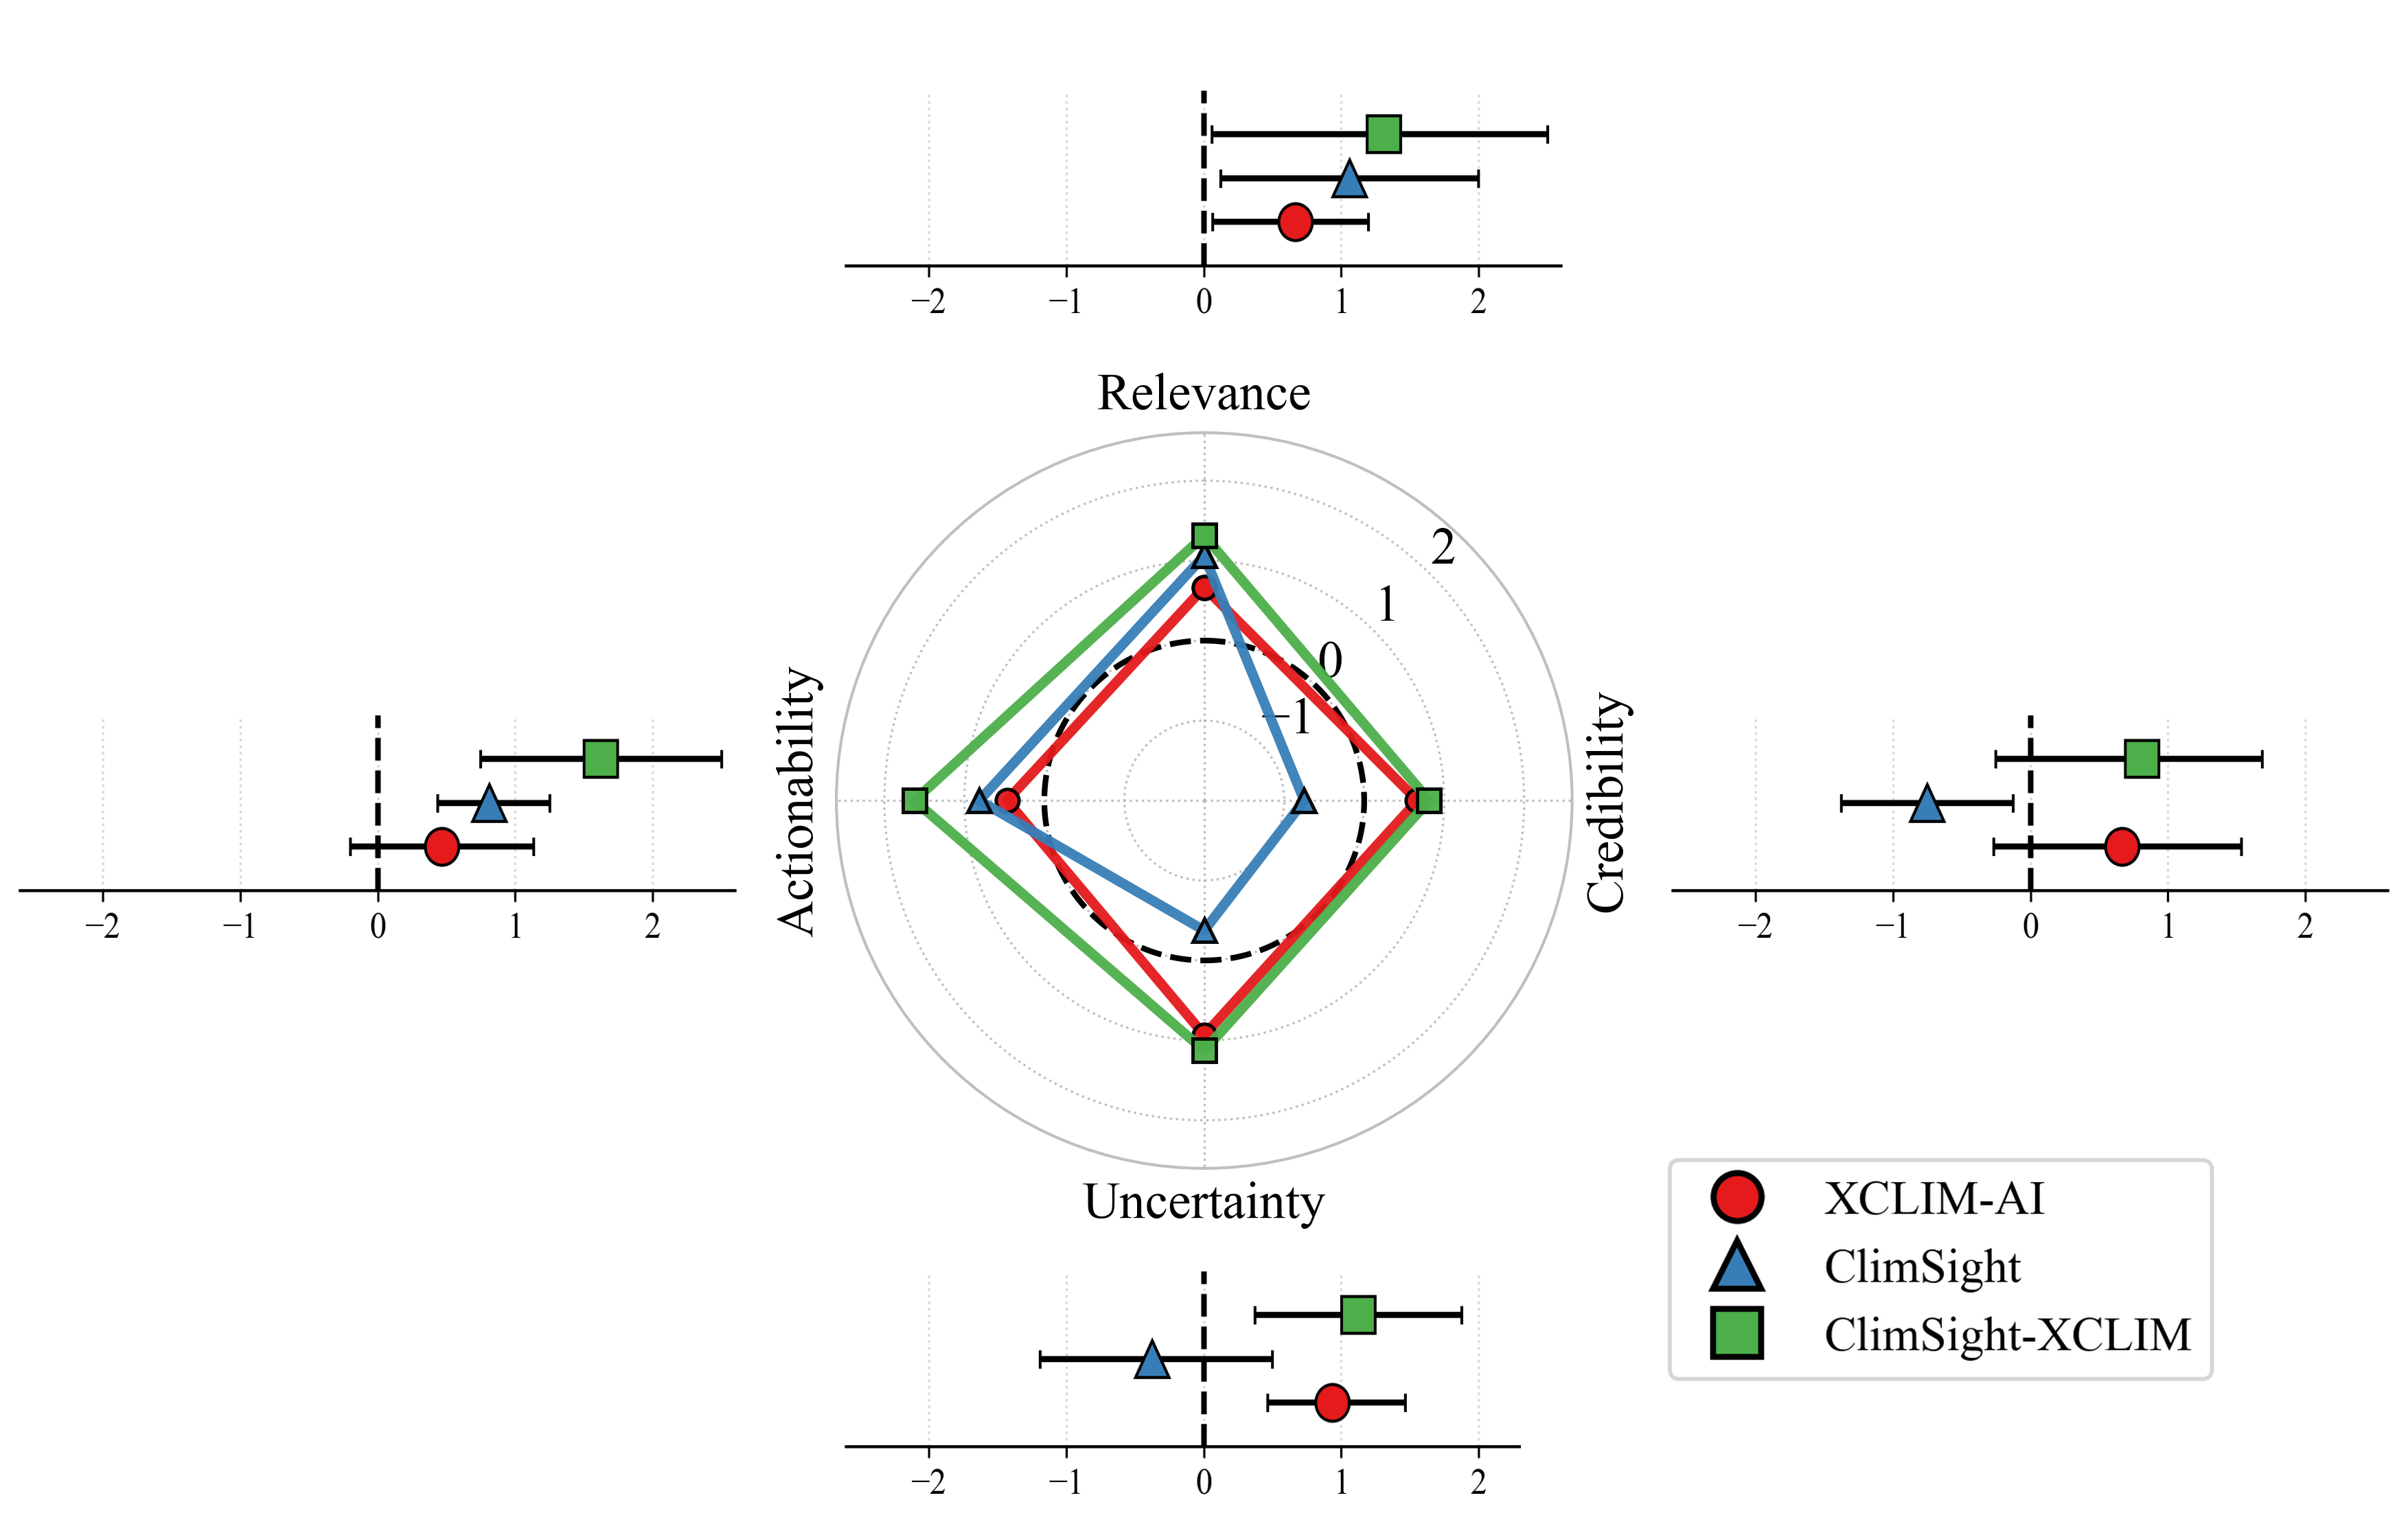
\includegraphics[
            width=\textwidth,
            height=0.34\textheight,
            keepaspectratio
        ]{Chapter5/figs/combined_cardinal_human.png}
        \caption{Human evaluators.}
        \label{fig:combined-human}
    \end{subfigure}

    \vspace{0.5cm}

    \begin{subfigure}{0.9\textwidth}
        \centering
        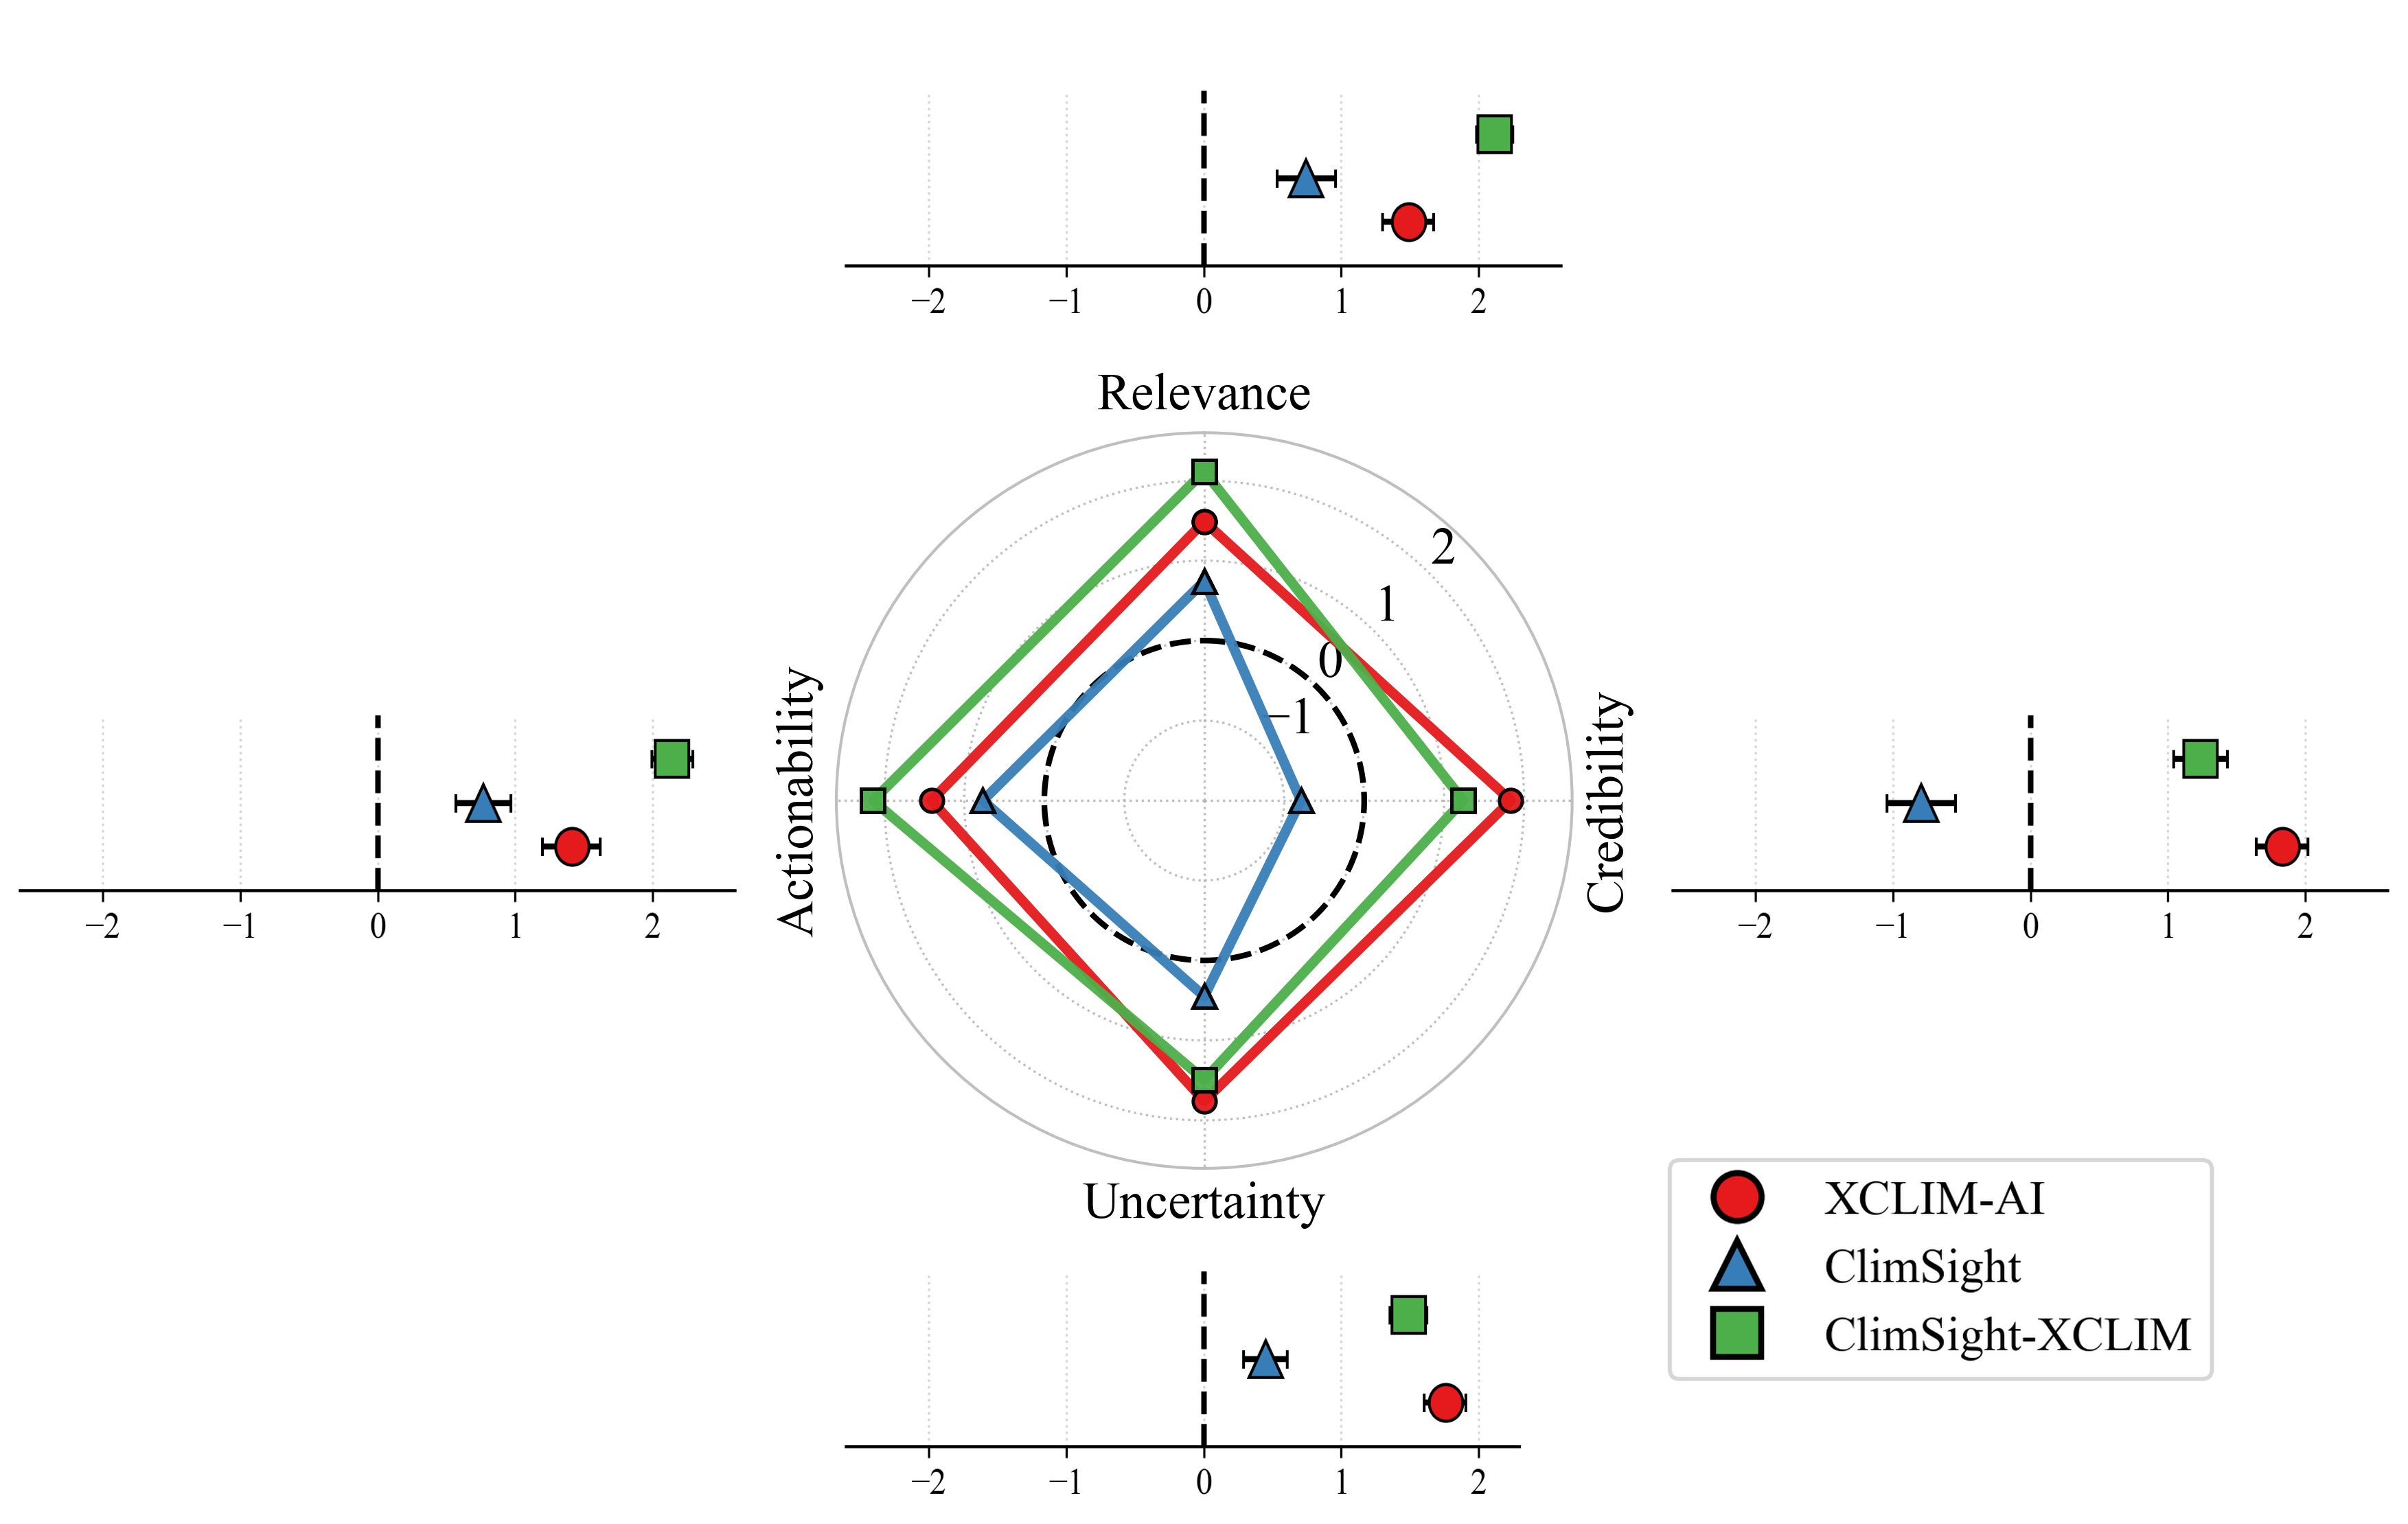
\includegraphics[
            width=\textwidth,
            height=0.34\textheight,
            keepaspectratio
        ]{Chapter5/figs/combined_cardinal_llm.png}
        \caption{LLMs as judges.}
        \label{fig:combined-llm}
    \end{subfigure}

    \caption{
        The central radar plot displays the average scores across all criteria, whereas the four subpanels show 95\% confidence intervals computed via a bootstrap procedure. For each metric we repeatedly drew 10{,}000 new samples from the original data and calculated the mean for each resample; the distribution of these bootstrap means was then used to derive the percentile bounds corresponding to a 95\% confidence level. The dashed line at $\Delta = 0$ highlights the point at which system performance equals that of the Plain-LLM baseline.
    }
    \label{fig:combined-cardinal}
\end{figure}

Figure~\ref{fig:combined-cardinal} report the aggregated scores collected during the evaluation. Human evaluation (Figure~\ref{fig:combined-human}) includes fewer ratings, as each question was assessed by a single expert. In contrast, all 22 LLM judges evaluated every answer (Figure~\ref{fig:combined-llm}), resulting in a much larger number of observations. This naturally leads to narrower 95\% confidence intervals for the LLM-based evaluation. Despite this difference in sample size, the overall patterns observed across the two evaluation methods are broadly consistent.

In both evaluations, all enhanced systems improve over the Plain-LLM baseline in terms of relevance and actionability.
The clearest gains are observed for ClimSight-XCLIM, which achieves the highest increase in actionability according to both human ($+1.6$) and LLM ($+2.1$) judges.
The same system also obtains a similar improvement in relevance, with closely aligned scores from LLM judges ($+2.1$) and human experts ($+1.3$).
Importantly, these effects are consistent: for ClimSight-XCLIM, the confidence intervals remain entirely above zero for both criteria and both evaluation methods.

The other two enhanced systems show a similar pattern, although less pronounced.
XCLIM-AI improves relevance in both evaluations, with median gains of $+0.7$ for human evaluators and $+1.5$ for LLM judges.
Its actionability gain is more clearly captured by the LLM-based evaluation ($+1.4$), while human evaluators assign a smaller increase ($+0.5$).
This latter value represents the only case in relevance and actionability where the confidence interval is not entirely positive, with a lower bound slightly below zero ($-0.2$).
ClimSight, instead, shows balanced improvements across the two criteria: relevance increases by $+1.1$ in the human evaluation and $+0.7$ in the LLM-based evaluation, while actionability improves by $+0.8$ in both cases.
As for ClimSight-XCLIM, all corresponding confidence intervals for ClimSight remain above zero, indicating that these improvements are stable across resampling.

Manual inspection of the generated responses shows that the Plain-LLM tends to produce outputs that are more vague and generic than those of the other systems, whereas the augmented models include more quantitative and context-specific statements, likely increase their perceived quality.

This observation is consistent with recent work on climate-oriented LLMs.
General purpose models can produce fluent and plausible climate explanations, but surface quality does not necessarily guarantee epistemic adequacy, factual grounding, or appropriate communication of uncertainty \citep{bulian_assessing_2024}.
Conversely, approaches that connect LLMs to authoritative climate sources, retrieval systems, and structured climate datasets have been proposed as a way to improve reliability and provide more localized and contextualized responses \citep{vaghefi_chatclimate_2023}.

Our results support this interpretation. The improved relevance and actionability of the enhanced systems appear to derive from their ability to anchor responses in retrievable evidence and computationally derived climate indicators. Notably, ClimSight-XCLIM, which combines both climate information retrieval and indicator computation, is also the system that achieves the highest perceived quality in relevance and actionability.

Our results on uncertainty and credibility highlight substantial disparities across systems. For uncertainty, XCLIM-AI and ClimSight-XCLIM show clear improvements over the Plain-LLM baseline in both evaluation settings.
Human evaluators assign median gains of $+0.9$ to XCLIM-AI and $+1.1$ to ClimSight-XCLIM, while LLM judges assign gains of $+1.8$ and $+1.5$, respectively. By contrast, ClimSight exhibits a weaker and less consistent pattern: human evaluators report a slight decrease in uncertainty expression ($-0.4$) with a lower 95\% confidence value of $-1.25$, whereas LLM judges assign only a small positive change ($+0.4$).

Credibility shows an even sharper separation between systems.
XCLIM-AI improves credibility according to both human evaluators ($+0.7$) and LLM judges ($+1.8$), and ClimSight-XCLIM follows the same positive trend, with gains of $+0.8$ and $+1.2$, respectively.
However, in the human evaluation, the confidence intervals for both XCLIM-AI and ClimSight-XCLIM extend slightly below zero, indicating some uncertainty around the magnitude and stability of these positive effects.
By contrast, the LLM-based evaluation assigns entirely positive confidence intervals to both systems. ClimSight, however, is the only system that deteriorates in credibility across both evaluation methods, with median $\Delta$ scores of $-0.8$ for both human evaluators and LLM judges. This negative effect is stable across resampling, as the confidence intervals remain entirely below zero in both evaluations.

General purpose LLMs can produce coherent and plausible explanations, but they remain prone to hallucination and to weaknesses in factual grounding, specificity, completeness, and uncertainty communication \citep{ji_survey_2023, bulian_assessing_2024}.
This is particularly consequential in climate-related domains, where scientific claims often depend on model uncertainty, scenario assumptions, confidence levels, spatial resolution, and evolving evidence.
In such contexts, credibility depends not only on the fluency of the answer, but also on whether claims can be traced to reliable evidence and to a transparent process of knowledge production.

The credibility results can be interpreted in this light.
The Plain-LLM baseline may appear credible because it can generate fluent explanations and plausible citations ad hoc, even when the evidential basis of specific claims is weak or unverifiable.
Retrieval-based systems such as ClimSight are instead constrained by the sources actually available to them.
When these sources are incomplete, indirect, or insufficiently specific to the user query, the system has fewer opportunities to project unsupported confidence.
As a result, it may appear less credible than the Plain-LLM, not necessarily because it is less grounded, but because its grounding exposes the limits of the available evidence.

This interpretation is consistent with work on attribution in natural language generation, which argues that claims about the external world should be evaluated according to whether they are supported by identifiable sources \citep{rashkin_measuring_2022}.
It is also aligned with climate-oriented QA systems, where grounding LLMs in authoritative sources such as IPCC AR6 has been proposed as a way to reduce hallucination and outdated information while improving the reliability of climate answers \citep{vaghefi_chatclimate_2023}.
However, our results indicate that adding contextual or retrieved information is not, by itself, sufficient to improve credibility.
What matters is also whether the system can make clear how the evidence supports the conclusions it presents.

The stronger performance of XCLIM-AI and ClimSight-XCLIM suggests that climate indicator computation adds a different form of grounding.
In these systems, part of the answer is supported by indicators computed from climate model data through an explicit analytical workflow.
The resulting claims are therefore not only textually grounded, but procedurally grounded: they are connected to indicator definitions, parameter choices, model data, and deterministic calculations.
This provides a stronger basis for quantitative statements and helps explain why XCLIM-AI-based systems improve both perceived credibility and uncertainty communication, while ClimSight improves relevance and actionability but not credibility to the same extent.

\subsection{Agreement Between Human and LLM Evaluators} \label{agreement}

\begin{figure}[H]
    \centering
    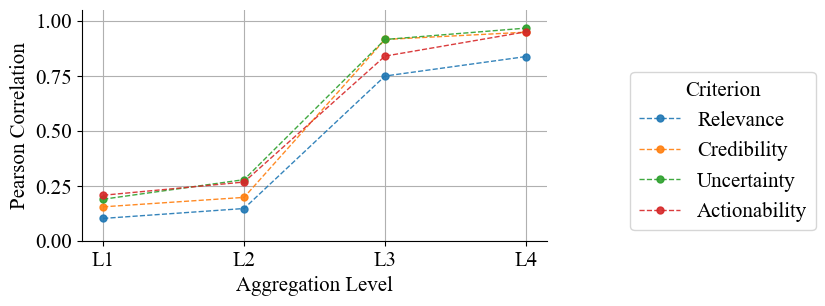
\includegraphics[width=1\textwidth]{Chapter5//figs/icc_evolution.png}
    \caption{
        Human--LLM agreement across increasing levels of aggregation. Pearson correlations are computed between human and LLM-assigned $\Delta$-scores for each evaluation criterion. L1 compares individual human judgments with single-LLM judgments at the question level; L2 averages LLM judgments across judges while preserving question-level comparisons; L3 aggregates scores at the system level for each individual LLM judge; and L4 compares system-level averages after aggregating across both questions and LLM judges.
        }

    \label{fig:icc-levels}
\end{figure}

Our evaluation framework employs 22 LLMs as judges and was designed to reduce judge-specific bias while producing meaningful comparisons with human assessments. In this section, we quantify the agreement between the $\Delta$-scores assigned by the ensemble of LLM judges and those assigned by human evaluators. To this end, we compute the Pearson correlation coefficient between human and LLM-assigned scores at four different levels of aggregation (Figure~\ref{fig:icc-levels}):

\begin{enumerate}
    \item \textbf{Level 1 (L1): Question-level, single-LLM agreement.}
    At this level, each human judgment is compared directly with the score assigned by a single LLM judge on the same question and system.
    No aggregation is performed: every comparison involves one human score and one single-LLM score for each question–system pair.
    Agreement is low across all criteria due to strong item-level variability and judge-specific noise.

    \item \textbf{Level 2 (L2): Question-level, mean-LLM agreement.}  
    This level still operates at the question level, but LLM judgments are aggregated before comparison.  
    For each question–system pair, we compute the average score assigned by all LLM judges, and we compare this mean-LLM score with the corresponding human score.  
    This reduces variability across judges while preserving question-level resolution.  
    Agreement improves moderately.
    
    \item \textbf{Level 3 (L3): System-level, single-LLM agreement.}  
    At this level, we aggregate across questions instead of across judges.  
    For each system, we compute the average human score over all its questions, and we separately compute the average score assigned by each single LLM judge across the same questions.  
    These system-level averages are then compared.  
    Removing item-level noise leads to a sharp increase in agreement.
    
    \item \textbf{Level 4 (L4): System-level, mean-LLM agreement.}  
    This is the most aggregated setting.  
    For each system, we compare the human average across all questions with the average score assigned by all LLM judges, also aggregated across all questions.  
    This combines both forms of aggregation—across judges and across items—and yields the highest agreement across all criteria.
\end{enumerate}

These results show that removing question-to-question variability substantially increases the alignment between LLM judges and human evaluators.
Once scores are aggregated at the system level, even a single-LLM judge already provides a reliable approximation of human assessments.
When the mean-LLM score is used, the agreement becomes remarkably high, with Pearson correlations above 0.95 for all criteria (except relevance, which still exhibits a strong correlation of 0.84).
It should be noted, however, that removing question-level variability implies that the agreement is measured over differences between system-level performance profiles rather than over individual questions.

Overall, these findings suggest that LLM-as-a-judge is highly effective when evaluations are aggregated over multiple items, as aggregation cancels out the substantial noise present in single-question judgments.
However, at the level of individual questions, single-LLM judgments remain unreliable, and their use should therefore be restricted to settings where either ensembles (mean-LLM) or item-level aggregation are feasible.

\section{Discussion}

The results of this chapter address two related questions: how different forms of augmentation change the contribution of LLMs to Climate Services, and how these changes can be evaluated. The main conclusion is that augmentation does not improve all dimensions of epistemic quality equally. Contextual augmentation primarily increases the specificity and practical orientation of responses, whereas computational augmentation provides a stronger basis for quantitative claims. Their combination produces the most consistent improvements, although its effectiveness remains dependent on how the different sources of evidence are integrated within the system architecture. The transition from climate information to knowledge therefore depends not simply on how much information is supplied to the model, but on how that information is produced, connected, and communicated.

The most distinctive contribution of computational augmentation can be described as \emph{procedural grounding}. Textual grounding connects a statement to an identifiable source; procedural grounding additionally connects a quantitative claim to the data, indicator definition, parameters, and analytical procedure through which it was obtained. This establishes a clearer boundary between computed evidence and model inference. 

Nevertheless, computation alone does not transform information into knowledge. A climate indicator becomes meaningful only when interpreted in relation to the exposed system and the decision under consideration. An earlier last spring frost may appear favourable for vineyards, but concurrent changes in budburst can preserve or increase frost vulnerability. Similarly, a projected change in precipitation extremes cannot by itself determine the additional capacity required for an urban drainage system. Procedural and contextual grounding are therefore complementary: the former produces traceable climate information, while the latter connects it to impacts, vulnerabilities, and possible responses.

These observations also demonstrate why conventional evaluations of LLMs are insufficient for Climate Services. Factual correctness and linguistic fluency remain important, but they do not establish whether a response is usable within a specific decision context. An answer may be plausible but geographically irrelevant, quantitatively precise but poorly justified, or scientifically grounded without providing a meaningful interpretation for the user. The four dimensions adopted in this chapter (relevance, credibility, uncertainty communication, and actionability) make these differences explicit and capture complementary attributes of usable climate knowledge. Since different forms of augmentation affect these dimensions in different ways, the same criteria can also inform system design: credibility requires traceable evidence and transparent analytical choices; uncertainty communication requires assumptions, model spread, scenarios, and data limitations to be preserved; and relevance and actionability require climate information to be interpreted in relation to the user's context and decision problem.

The comparison between human and automated evaluations provides a further methodological insight. LLM judges reproduce the overall direction of human assessments reasonably well when their scores are aggregated across questions and evaluators. They can therefore support the comparison of alternative architectures or augmentation strategies during system development. Their agreement with human evaluators is substantially weaker for individual responses, however, and aggregation cannot demonstrate that a judge has correctly assessed the suitability of a specific indicator or recommendation. LLM-based evaluation should therefore be treated as a system-level development instrument rather than as a mechanism for certifying individual Climate Service outputs.

From an operational perspective, systems such as XCLIM-AI can reduce the technical distance between questions expressed in operational language and the indicators, datasets, and procedures required to address them. They could support indicator exploration, preliminary climate risk assessments, comparisons between historical and future conditions, and the preparation of technical reports. They may also facilitate communication between scientists and users by translating practical questions into formal analyses and numerical outputs into accessible explanations.

Several limitations condition these conclusions. The evaluation is based on 50 localized adaptation questions covering ten thematic categories and cannot represent the full diversity of Climate Services. In addition, GPT-4.1 was used as the backbone of all four systems. This choice isolates the contribution of augmentation, but limits the generalizability of the results to models with different tool-use and reasoning capabilities. The XCLIM-AI implementation also represents only one configuration of computational augmentation, constrained by the indicators available in \emph{xclim}, the variables accessible through Open-Meteo, seven HighResMIP models, a selected scenario and set of time periods, and point-based spatial extraction. Operational applications may require observations, additional scenarios, downscaled projections, impact models, and spatial aggregation.

The study evaluates the final responses without independently scoring every component of the analytical chain. It is therefore not always possible to determine whether a weakness originates from indicator retrieval, parameter selection, tool execution, numerical interpretation, or final synthesis. Moreover, the framework measures perceived epistemic quality rather than providing complete verification of scientific correctness. Each question was evaluated by one human expert, while the LLM judges are neither statistically nor epistemically independent. Finally, the experiment concerns fully automated workflows and assesses actionability as a property of the generated text, rather than through its effects on actual decisions. Future work should combine end-to-end evaluation with component-level validation and examine these systems within collaborative Climate Service processes.